\subsubsection{Screens}Zur besseren Übersichtlichkeit hat sich das Projektteam entschieden, die App zuerst in Englisch zu entwickeln.\\

\paragraph{Home}Mit der Funktion UseEffect, die am Rendern des Screens ausgeführt wird, wird die Funktion UserStatus ausgeführt.\\
Die Funktion UserStatus überprüft, ob die anwendende Person angemeldet ist. Falls die anwendende Person nicht angemeldet ist, wird eine Aufforderung zur Anmeldung angezeigt (siehe Abbildung x). Falls der die anwendende Person angemeldet ist, wird die Funktion getActivity() ausgeführt. \\
Die Funktion getActivity() wird verwendet, um alle Buchungen der anwendenden Person abzufragen. Falls die Buchungen in der Vergangenheit liegen, werden sie im Array FormerList gespeichert, wenn das Fahrrad noch gelagert ist, wird die Buchung im Array ActivityList gespeichert. \\
Die Buchungen werden auf zwei Listen anzeigt. Falls keine Buchung gefunden wurde, kommt der Text „no data“. \\
Mit einem Klick auf den „Aktualisieren Button“ in der rechten oberen Ecke, werden die Buchungen der anwendenden Person neu aus der Datenbank abgerufen.\\
\begin{figure}[H]
    \centering
    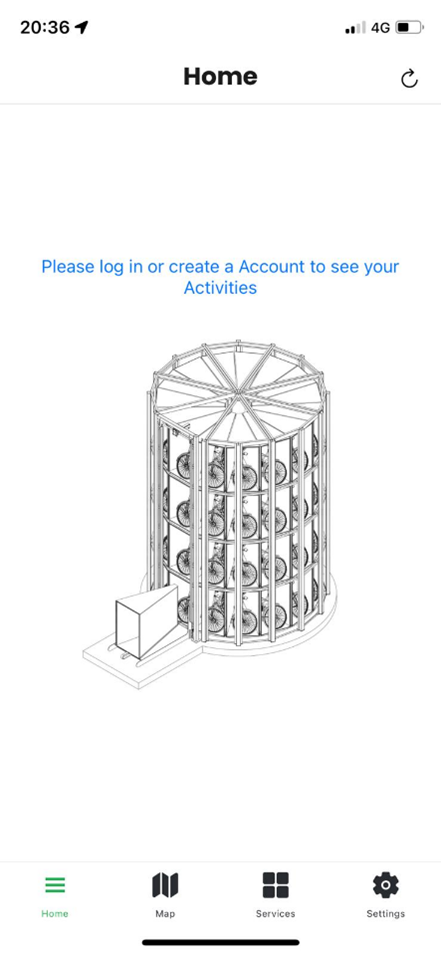
\includegraphics[width=0.25\textwidth]{images/app-screenshots/screenhomeno.png}
    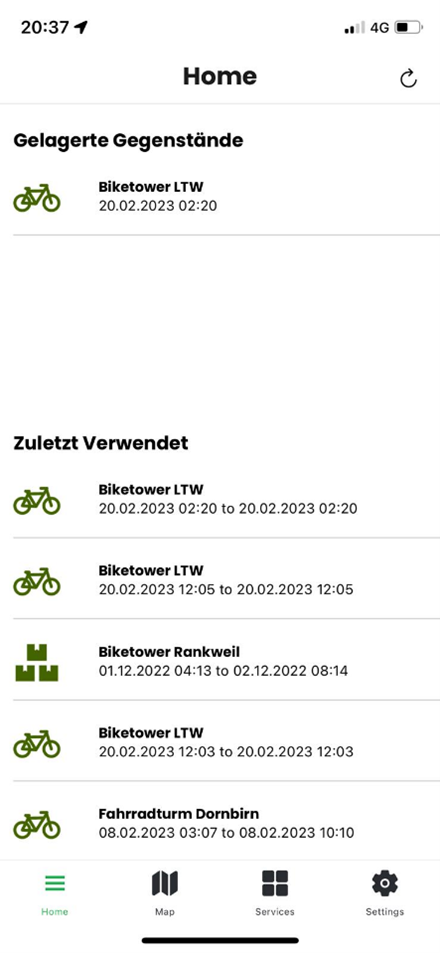
\includegraphics[width=0.25\textwidth]{images/app-screenshots/screenhomeyes.png}
    \caption{Screen Home}
    \label{fig:screenhome}
\end{figure}
Die Abbildung \ref{fig:screenhome} zeigt links die Ansicht ohne Anmeldung und rechts die Ansicht mit Anmeldung.


\paragraph{BoxInfo}
Auf dem Screen BoxInfo werden folgende Daten angezeigt:\\
\begin{itemize}
    \item Name des Fahrradparkhauses in dem sich die Box befindet
    \item Beginn der Buchung und falls die Buchung in der Vergangenheit liegt, zusätzlich die Zeit der Abholung
    \item Komponente BoxImage für Bild der Fahrradbox
\end{itemize}
Diese Infos werden über die Navigation übergeben.\\ 
\begin{minted}{js}
    navigation.navigate("boxinfo", { box: this.props.boxinfo })
\end{minted}
Der Code zeigt, wie man von der Komponente Box zum aktuellen Screen navigiert wird. Dort wird das Array boxinfo übergeben.\\
\begin{minted}{js}
    export default function BoxInfo({ route, navigation }) {
    const { box } = route.params;
    ...}
\end{minted}
Beim aktuellen Screen wird nun die Variable Box mithilfe von route.params abgerufen. \\ \\
Falls man das Fahrrad noch nicht abgeholt hat, wird außerdem ein Button zum Auslagern angezeigt. Durch das Drücken des Buttons kommt man zum Screen Assignment.\\
\begin{figure}[H]
    \centering
    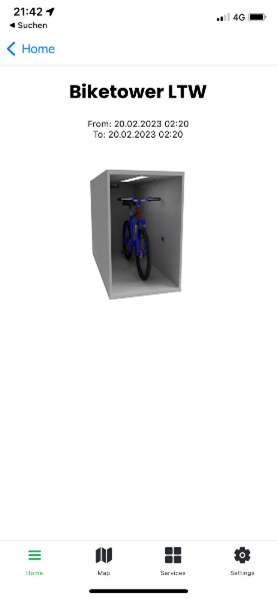
\includegraphics[width=0.25\textwidth]{images/app-screenshots/screenboxinfo.png}
    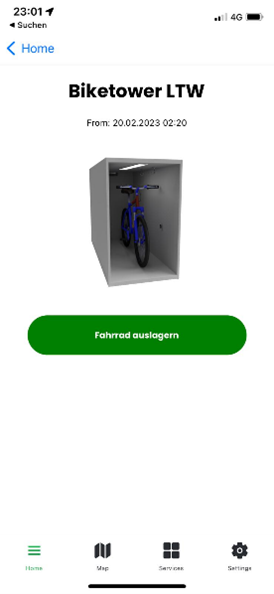
\includegraphics[width=0.25\textwidth]{images/app-screenshots/screenboxinfov.png}
    \caption{Screen BoxInfo}
    \label{fig:screenboxinfo}
\end{figure}
Die Abbildung \ref{fig:screenboxinfo} zeigt links die Ansicht bei einer bereits vergangenen Buchung und rechts die Ansicht bei einer aktiven Buchung.\\


\paragraph{Assignment}

\paragraph{Services}Beim Screen Services werden verschiedene Dienstleistungen angezeigt. Dafür wird die Komponente OtherLink verwendet, mit der man zu einer Unterseite gelangt.\\
\begin{figure}[H]
    \centering
    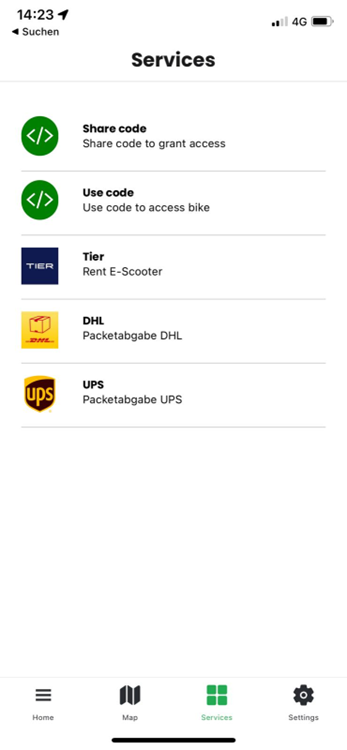
\includegraphics[width=0.25\textwidth]{images/app-screenshots/screenservices.png}
    \caption{Screen Services}
    \label{fig:screenservices}
\end{figure}


\paragraph{Settings}Der Screen Settings wird zur Verlinkung auf diverse Unterseiten verwendet. Dafür wird die Komponente SettingLink mehrmals verwendet.\\
Mit der Funktion UserStatus wird überprüft, ob die anwendende Person angemeldet ist und dementsprechend andere Einstellungen angezeigt. \\
\begin{figure}[H]
    \centering
    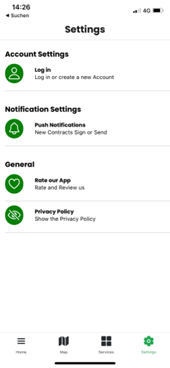
\includegraphics[width=0.25\textwidth]{images/app-screenshots/screensettingsa.png}
    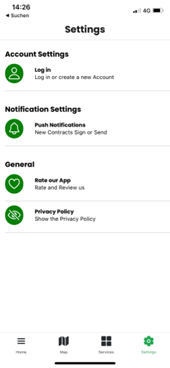
\includegraphics[width=0.25\textwidth]{images/app-screenshots/screensettingsa.png}
    \caption{Screen Settings}
    \label{fig:screensettings}
\end{figure}
Die Abbildung links zeigt die Ansicht, wenn die anwendende Person nicht angemeldet ist. Bei der Abbildung rechts sieht man, dass mehrere Einstellungen zum Account angezeigt werden, falls die anwendende Person eingeloggt ist. \\


\paragraph{LogIn}Der Screen LogIn dient zum Anmelden mit einem bestehenden Account. Im Screen LogIn gibt es zwei Textfelder zum Eingeben der E-Mail und des Passworts. \\
Mit einem Klick auf den Button „Sign in“ wird die Funktion SignIn ausgeführt. \\
\begin{minted}{js}
    function SignIn() {
    auth
      .signInWithEmailAndPassword(email, password)
      .then((userCredential) => {
        setError("")
        const user = userCredential.user;
        Alert.alert("signed in");
        navigation.navigate("settings", {created: false});
      })
      .catch((error) => {
        const errorCode = error.code;
        const errorMessage = error.message;
        setError(errorMessage)
      });
  };
\end{minted}

Dabei wird die Methode signInWithEmailAndPasswort des Authentizierungs-Service auth von Firebase verwendet. Es werden die eingegebene E-Mail und Passwort übergeben. Bei einer erfolgreichen Anmeldung bekommt die anwendende Person die Meldung „signed in“ und wird zum Screen „Settings“ zurückgeleitet.\\
Beim Klicken auf den Button „Register“ wir man zur Seite SignIn geführt.\\


\paragraph{SignIn}Der Screen SignIn dient zum Erstellen eines Accounts. In den Textfeldern kann man den eigenen Namen, die E-Mail und ein Passwort eingeben.\\
Wenn man auf den button „create Account“ klickt, wird die Funktion createAccount ausgeführt.\\
\begin{minted}{js}
   function createAccount() {
    auth
      .createUserWithEmailAndPassword(email, password)
      .then(() => {
        setError("")
        addUser(auth.currentUser.uid,email,name)
        Alert.alert("User signed in and logged in");
        navigation.navigate("settings", { created: true, name: name});
      })
      .catch((error) => {
        if (error.code === "auth/email-already-in-use") {
         setError("That email address is already in use!");
        }

        else if (error.code === "auth/invalid-email") {
          setError("That email address is invalid!");
        }
        else {
        setError(error.message);
        }
      });
  };
\end{minted}

Die Methode createUserWithEmailAndPasswort, die zum Erstellen eines Users verwendet wird, ist vergleichbar mit signInWithEmailAndPasswort. Sie erstellt beim Authentifizierungs-Service auth einen neuen User und meldet diesen an. Falls die Erstellung des Accounts erfolgreich ist, werden folgende Schritte ausgeführt:
\begin{itemize}
    \item Die Funktion addUser wird ausgeführt. Damit wird für den User in Firestore ein Dokument mit dem Namen und der userid erstellt. 
    \item Ausgabe der Meldung "User signed in and logged in".
    \item Die anwendende Person wird zurück zu Settings navigiert.
\end{itemize}
Falls die Erstellung des Accounts nicht möglich ist, wird eine entsprechende Fehlermeldung ausgegeben.\\

\paragraph{Map}Auf dem Screen Map werden die Standorte von Fahrradparkhäusern angezeigt.\\
Mithilfe vom Expo SplashScreen wird zuerst eine leere Karte angezeigt, bis die Funktion getTowers fertig ist. Die Funktion getTowers liefert die Daten zu allen Fahrradtürmen. \\
Anschließend werden alle Marker auf der Karte angezeigt. Die Funktion MarkerImage liefert entweder einen grüner Marker, falls noch Plätze frei sind, oder einen grauen Marker wenn es keine freien Plätze gibt. Beim Klicken auf einen Marker, kommt man zum Screen TowerInfo.\\

\begin{figure}[H]
    \centering
    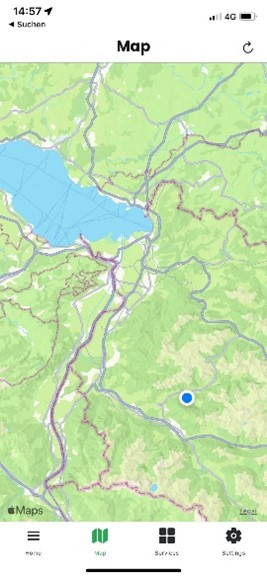
\includegraphics[width=0.25\textwidth]{images/app-screenshots/screenmapa.jpg}
    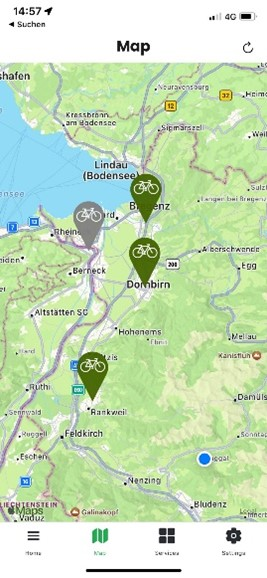
\includegraphics[width=0.25\textwidth]{images/app-screenshots/screenmapb.jpg}
    \caption{Screen Map}
    \label{fig:screenmap}
\end{figure}

Die Abbildung links zeigt die Karte, wenn die Türme noch nicht aus der Datenbank geladen sind.
Auf der Abbildung rechts sieht man eine Karte mit vier Beispiel-Türmen. Der Turm links oben ist grau, da dort kein Platz frei ist. \\
